\appendix

\chapter{Appendix} \label{chapter:appendix}

\section{Source-Code}
The source code of the thesis is available on GitHub split in two repositories: 
Evaluation repository with Prototype:\\
\url{https://github.com/justingebert/quixbugs-apr}\\
Prototype: \url{https://github.com/justingebert/bugfix-ci}


\newpage

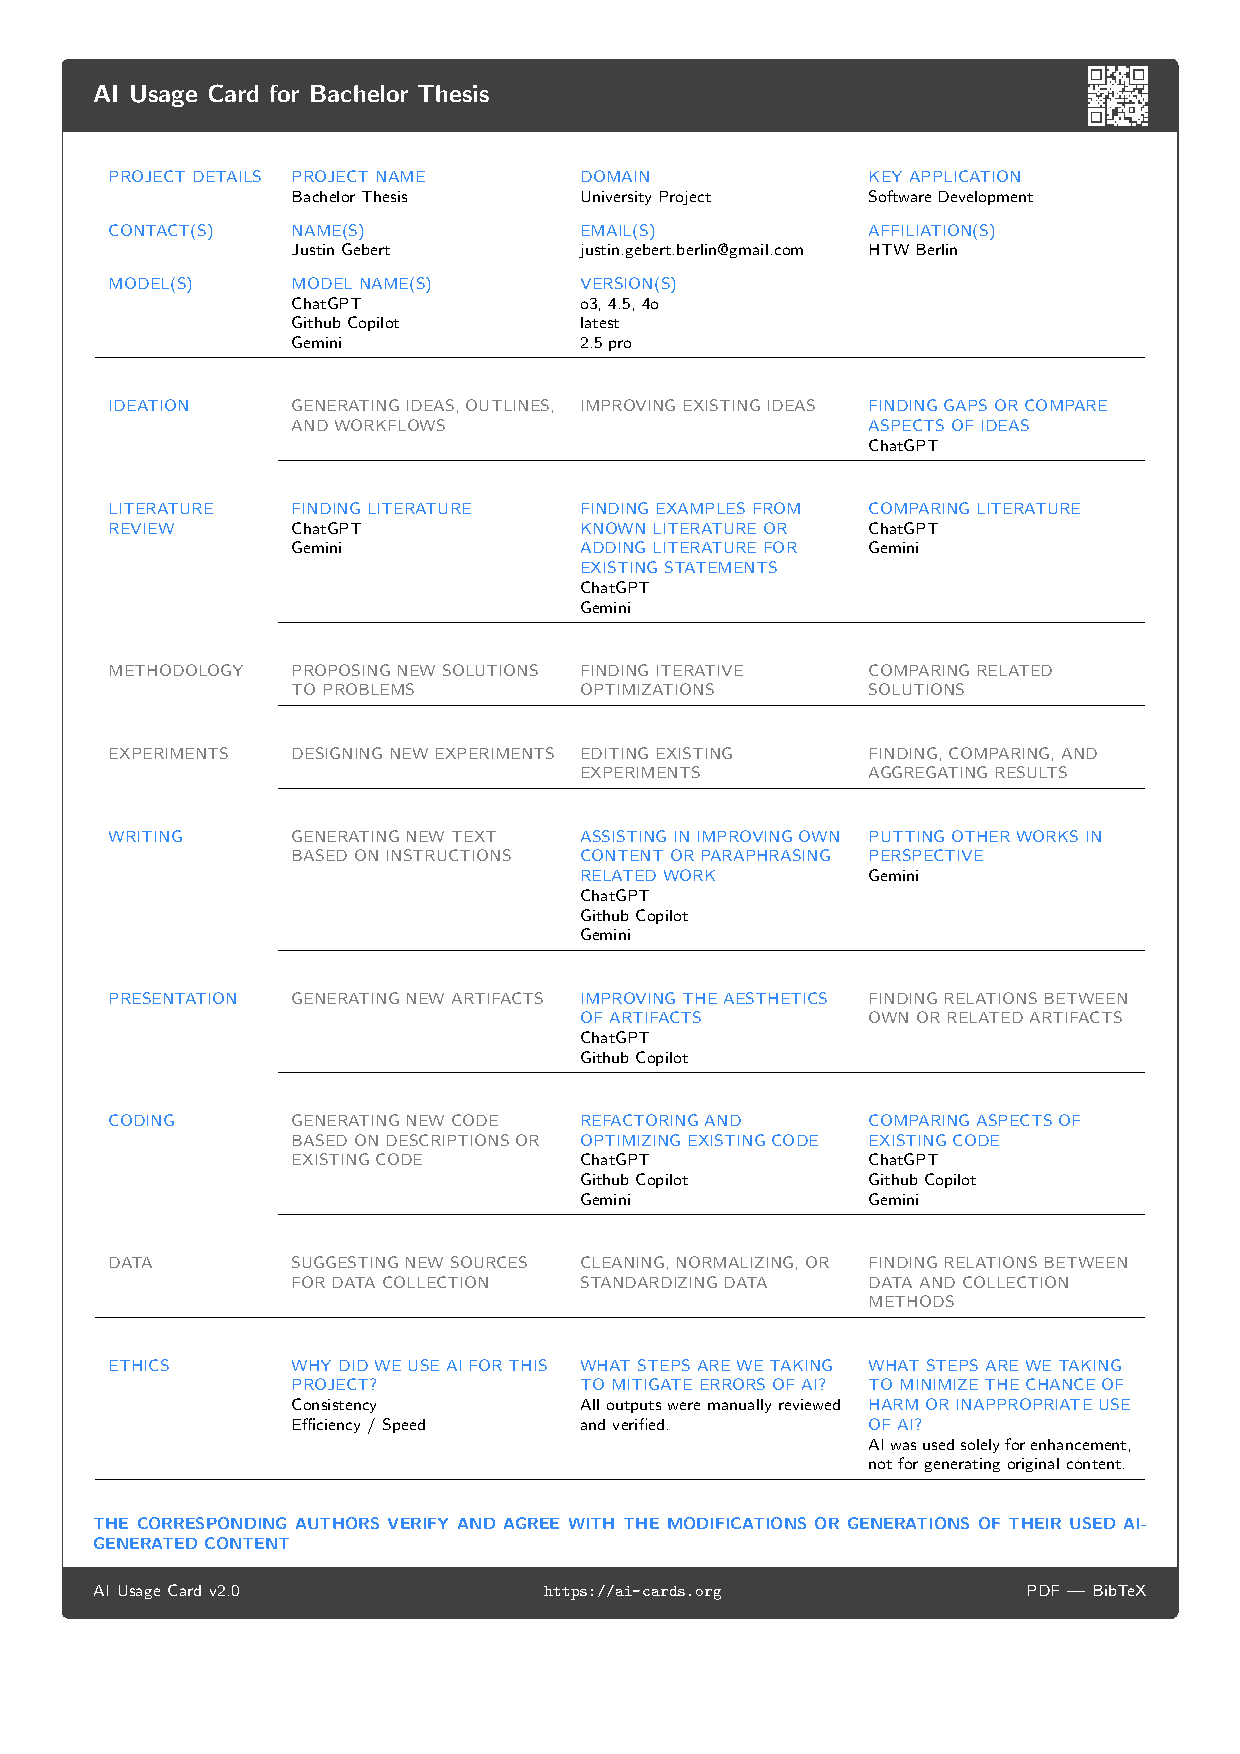
\includepdf[pages={1}]{pages/Ai-usage-card.pdf}

\thispagestyle{empty}
%\vspace*{18cm}
\noindent


\section*{Eidesstattliche Versicherung}
Hiermit versichere ich an Eides statt durch meine Unterschrift, dass ich die vorstehende Arbeit selbstst\"andig und ohne fremde Hilfe angefertigt und alle Stellen, die ich w\"ortlich oder ann\"ahernd w\"ortlich aus Ver\"offentlichungen entnommen habe, als solche kenntlich gemacht habe, mich auch keiner anderen als der angegebenen Literatur oder sonstiger Hilfsmittel bedient habe. Die Arbeit hat in dieser oder \"ahnlicher Form noch keiner anderen Pr\"ufungsbeh\"orde vorgelegen.\\
\linebreak[4]
\linebreak[4]
\linebreak[4]
\linebreak[4]
-------------------------------------------------------\linebreak[4]
Datum, Ort, Unterschrift